%-----------------------------------------------------------------------------%
\chapter{\babDua}
\label{bab:2}


\section{Masalah Pemeringkatan Teks}
    Permasalahan pemeringkatan teks adalah Permasalahan untuk menentukan urutan dokumen yang paling relevan dengan kueri $q$ yang diberikan. Dalam bahasa yang lebih formal, diberikan kueri $q$ dan himpunan dokumen terbatas $\mathcal{D}= \{d_1, d_2, ..., d_n\}$, keluaran yang diinginkan dari permasalahan ini adalah barisan dokumen $D_k = (d_{i_1}, d_{i_2}, ..., d_{i_k})$ yang merupakan $k$ dokumen yang paling relevan dengan kueri $q$. Selain itu, biasanya nilai $k$ akan lebih kecil dari banyaknya dokumen yang ada, sehingga permasalahan pemeringkatan sering juga disebut sebagai \f{top-k retrieval}. Untuk mengukur performa suatu model pemeringkatan, biasanya digunakan metrik evaluasi seperti presisi, \f{recall}, \f{reciprocal rank}, dan \f{normalized discounted cumulative gain} (nDCG) yang akan dijelaskan pada \sect~\ref{sec:metrik-evaluasi}.

    \subsection{Bentuk Umum \f{Dataset}}
    \label{sec:dataset-umum}
    Sebelum menjelaskan metrik evaluasi, akan dijelaskan terlebih dahulu bentuk umum dari \f{dataset} yang digunakan untuk mengevaluasi sebuah sistem pemeringkatan teks. Bentuk umum dari \f{dataset} yang digunakan biasanya terdiri dari 3 \f{file}, yaitu \f{file} korpus, \f{file} kueri, dan \f{file judgements}. \f{File} korpus adalah kumpulan dokumen/teks yang ingin di-\f{retreive} oleh sebuah sistem pemeringkatan teks. Biasanya, pada \f{file} korpus terdapat 3 kolom, yaitu id teks, judul teks, dan isi dari teks tersebut. \tab~\ref{tab:contoh-file-korpus} menunjukkan potongan dari \f{file} korpus.
    \begin{table}
        \centering
        \caption{Potongan \f{file} korpus \f{dataset} MIRACL.}
        \label{tab:contoh-file-korpus}
        \begin{tabular}{|l|l|p{0.6\textwidth}|}
            \hline
            \textbf{\_id}    & \textbf{title}             & \textbf{text}                                                                                                 \\ \hline
            1342516\#1  & Colobothea biguttata & Larva kumbang ini biasanya mengebor ke dalam kayu dan dapat menyebabkan kerusakan pada batang kayu hidup atau kayu yang telah ditebang. \\ \hline
            1342517\#0  & Ichthyodes rufipes  & Ichthyodes rufipes adalah spesies kumbang tanduk panjang yang berasal dari famili Cerambycidae. Spesies ini juga merupakan bagian dari genus Ichthyodes, ordo Coleoptera, kelas Insecta, filum Arthropoda, dan kingdom Animalia. \\ \hline
        \end{tabular}
    \end{table}

    \f{file} kueri berisi kumpulan kueri yang digunakan untuk mengambil dokumen dari \f{file} korpus. 
    performa dari sistem pemeringkatan teks akan diukur dengan mengambil $k$ dokumen dari \f{file} korpus untuk setiap kueri pada \f{file} kueri. Biasanya, pada \f{file} kueri terdapat 2 kolom, yaitu id kueri dan isi dari kueri tersebut. \tab~\ref{tab:query-file-example} menunjukkan potongan dari \f{file} kueri.
    \begin{table}
        \centering
        \caption{Potongan \f{file} kueri \f{dataset} MIRACL.}
        \label{tab:query-file-example}
        \begin{tabular}{|l|p{0.8\textwidth}|}
            \hline
            \textbf{\_id} & \textbf{text}                                                                 \\ \hline
            3             & Dimana James Hepburn meninggal?                                              \\ \hline
            4             & Dimana Jamie Richard Vardy lahir?                                            \\ \hline
            11            & berapakah luas pulau Flores?                                                 \\ \hline
            17            & Siapakah yang menulis Candy Candy?                                           \\ \hline
            19            & Apakah karya tulis Irma Hardisurya yang pertama?                              \\ \hline
        \end{tabular}
    \end{table}
    Selanjutnya \f{file judgements} berisi pemetaan relevansi antara kueri pada \f{file} kueri dengan dokumen pada \f{file} korpus. Biasanya, pada \f{file} judgements terdapat 3 kolom, yaitu id kueri, id dokumen, dan relevansi antara kueri dan dokumen tersebut ($r$). Pasangan $(\text{kueri}, \text{dokumen})$ yang relevan akan memiliki nilai $r > 0$ dan nilai $r$ yang makin besar menunjukkan relevansi yang makin tinggi. Selain itu, pasangan $(\text{kueri}, \text{dokumen})$ yang tidak relevan akan memiliki nilai $r = 0$ dan biasanya pasangan $(\text{kueri}, \text{dokumen})$ yang tidak relevan tidak dituliskan pada \f{file judgements}. tak menutup kemungkinan jika sebuah \f{dataset} hanya menggunakan nilai relevansi biner ($r \in \{0, 1\}$). Terakhir, \tab~\ref{tab:judgements-file-example} menunjukkan potongan dari \f{file judgements}.
    \begin{table}
        \centering
        \caption{Potongan \f{file} judgements \f{dataset} MIRACL.}
        \label{tab:judgements-file-example}
        \begin{tabular}{|l|l|l|}
            \hline
            \textbf{query-id} & \textbf{corpus-id} & \textbf{score} \\ \hline
            3                 & 115796\#6          & 1              \\ \hline
            3                 & 77689\#48          & 1              \\ \hline
            4                 & 1852373\#0         & 1              \\ \hline
        \end{tabular}
    \end{table}
    


    \subsection{Metrik Evaluasi dalam Pemeringkatan Teks}
    \label{sec:metrik-evaluasi}
    Subbab ini menjelaskan beberapa metrik evaluasi yang sering digunakan untuk mengukur performa dari sistem pemeringkatan teks. Metrik evaluasi yang akan dijelaskan adalah \f{recall}, presisi, \f{reciprocal rank}, dan \f{normalized discounted cumulative gain} (nDCG). Metrik tersebut digunakan untuk mengukur performa dari sistem pemeringkatan teks dengan mengambil $k$ dokumen dari \f{file} korpus pada satu kueri. Untuk mendapatkan performa dari sistem pemeringkatan teks secara keseluruhan, biasanya metrik evaluasi tersebut akan dihitung untuk setiap kueri pada \f{file} kueri dan kemudian diambil nilai rata-ratanya.

    \subsubsection{\f{Recall} dan Presisi}

        \begin{figure}
            \centering
            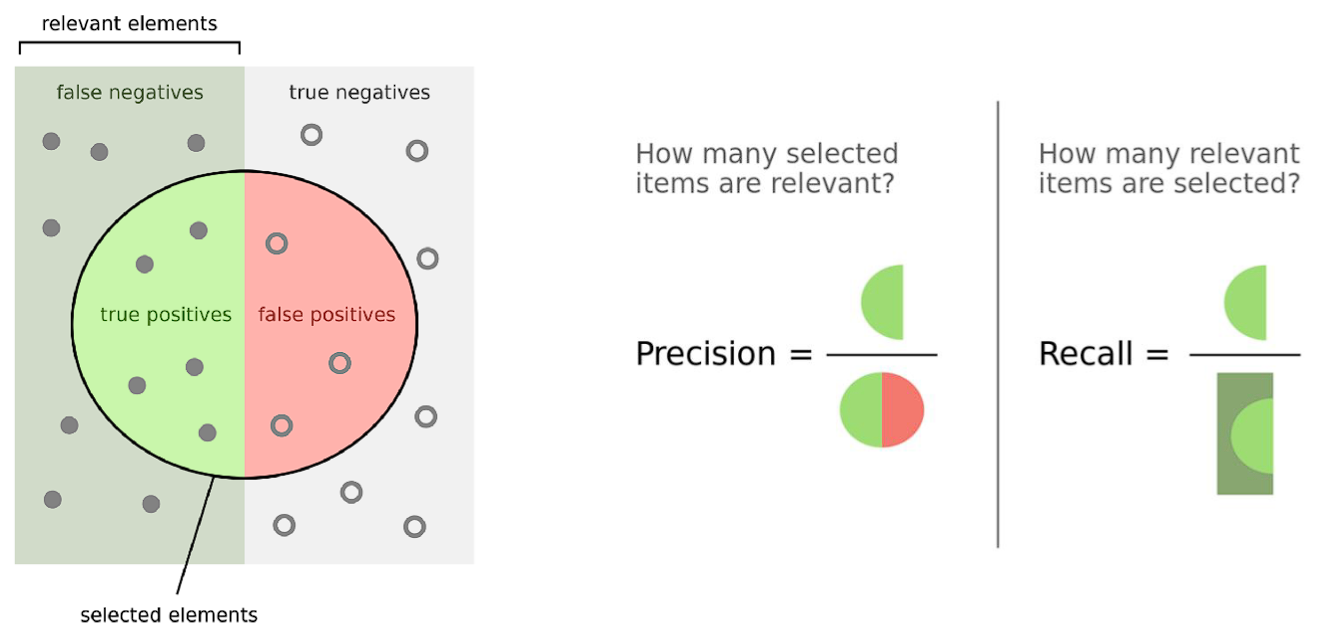
\includegraphics[width=1\textwidth]{assets/pics/recall-presisi.png}
            \caption{Ilustrasi \f{recall} dan presisi. Nilai \f{recall} dihitung sebagai rasio dokumen relevan yang diambil oleh sistem terhadap seluruh dokumen yang relevan dengan kueri $q$. Sedangkan nilai presisi dihitung sebagai rasio dokumen relevan yang diambil oleh sistem terhadap seluruh dokumen yang diambil oleh sistem.}
            \label{fig:recall-precision}
        \end{figure}
        Presisi dan \f{recall} adalah metrik yang paling sederhana untuk mengukur kemampuan dari suatu sistem pemeringkatan teks. \f{Recall} mengukur kemampuan sistem dalam mengembalikan semua dokumen yang relevan dengan kueri $q$ dari himpunan dokumen $\mathcal{D}$, sedangkan presisi mengukur kemampuan sistem dalam mengembalikan dokumen yang relevan dengan kueri $q$ dari himpunan dokumen $\mathcal{D}$. Untuk suatu kueri $q$, kumpulan dokumen $\mathcal{D} = \{d_1, d_2, ..., d_n\}$, dan barisan $k$ dokumen yang diambil oleh sistem, $D_k = (d_{i_1}, d_{i_2}, ..., d_{i_k})$, \f{recall} dan presisi dapat dihitung dengan \equ~\ref{eq:recall} hingga \equ~\ref{eq:presisi}.
        \begin{align}
            \label{eq:recall}
            \mathcal{D} &= \{d_1, d_2, \dots, d_n\} \\
            D_k &= (d_{i_1}, d_{i_2}, \dots, d_{i_k}) \\
            \text{recall}(q, D_k)\text{@k} &= \frac{\sum_{d \in D_k} \text{rel}(q, d)}{\sum_{d \in \mathcal{D}} \text{rel}(q, d)} \in [0, 1] \\
            \label{eq:presisi}
            \text{precision}(q, D_k)\text{@k} &= \frac{\sum_{d \in D_k} \text{rel}(q, d)}{|D_k|} \in [0, 1] \\
            \label{eq:rel}
            \text{dengan } \text{rel}(q, d) &= \begin{cases} 
            1 & \text{jika } r > 1 \\
            0 & \text{jika } r = 0
            \end{cases}        
        \end{align}

        Sebagai Contoh, Jika terdapat 10 dokumen yang relevan dengan kueri $q$, dan sistem mengembalikan $k=100$ dokumen, namun hanya terdapat 5 dokumen yang relevan pada $D_k$  maka \f{recall} dan presisi dari sistem tersebut adalah 0.5 ($\frac{5}{10}$) dan 0.05 ($\frac{5}{100}$) masing-masing. Baik \f{recall} maupun presisi memiliki rentang nilai dari 0 hingga 1, dengan nilai 1 menunjukkan performa sistem yang terbaik. perhitungan \f{recall} biasanya dilakukan untuk $k$ yang cukup besar ($k = 100,1000 $), sedangkan perhitungan presisi dilakukan untuk $k$ yang kecil ($k = 1, 3, 5$) \citep{irlecture}.


        \subsubsection{\f{Reciprocal Rank}}

        \begin{figure}
            \centering
            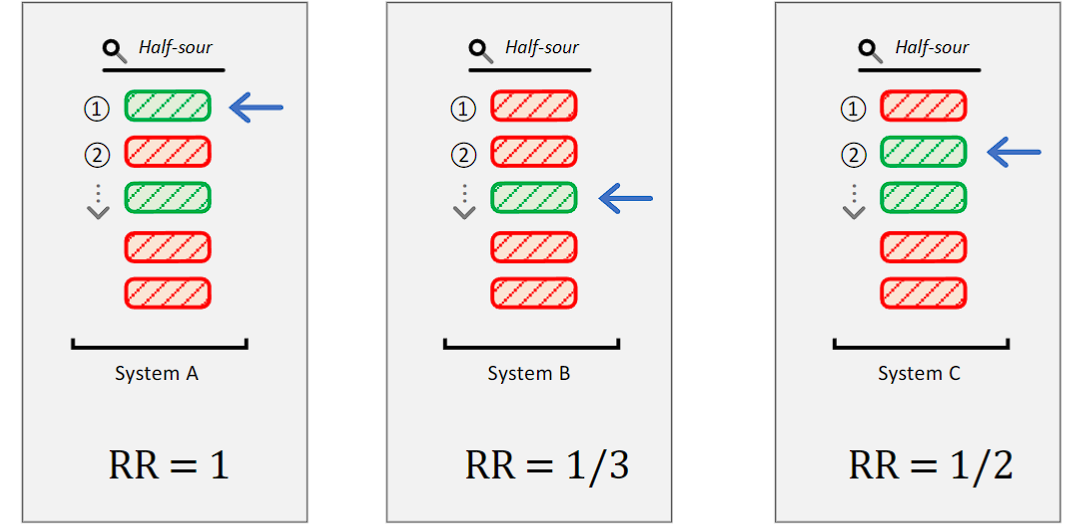
\includegraphics[width=1\textwidth]{assets/pics/rr.png}
            \caption{Ilustrasi \f{reciprocal rank}.}
            \label{fig:reciprocal-rank}
        \end{figure}
        Metrik lainnya yang sering digunakan untuk mengukur performa sistem pemeringkatan adalah \f{reciprocal rank} (RR). Metrik RR menitikberatkan pada peringkat dari dokumen relevan pertama dengan kueri $q$. \equ~\ref{eq:reciprocal-rank-start} hingga \equ~\ref{eq:reciprocal-rank-end} menunjukkan cara menghitung RR dari suatu kueri $q$ dan barisan $k$ dokumen yang diambil oleh sistem \citep{irlejcture, textrankingsurvey}.
        \begin{align}
            \text{RR}(q, D_k)\text{@k} &= \begin{cases}
                \label{eq:reciprocal-rank-start}
                \frac{1}{\text{FirstRank}(q, D_k)} & \text{jika } \exists d \in D_k \text{ dengan } \text{rel}(q, d) = 1 \\        
                0 & \text{jika } \forall d \in D_k, \text{ rel}(q, d) = 0 \\
                \end{cases} \in [0, 1] \\
                \label{eq:reciprocal-rank-end}
                \text{FirstRank}(q,D_k) &= \text{posisi dokumen relevan pertama } d\in D_k \text{ dengan } \text{rel}(q, d) = 1
        \end{align}

        \pic~\ref{fig:reciprocal-rank} mengilustrasikan metrik RR. Pada gambar tersebut, nilai RR dari sistem A adalah 1 $(\frac{1}{1})$ karena posisi dari dokumen yang relevan pertama adalah 1. Nilai RR dari sistem B dan sistem C masing-masing adalah  0.33 $(\frac{1}{3})$ dan 0.5 $(\frac{1}{2})$ karena posisi dari dokumen yang relevan pertama adalah 3 dan 2. Selain itu, jika tidak terdapat dokumen yang relevan dengan kueri $q$ pada $D_k$, nilai RR dari sistem tersebut adalah 0. 

    \subsubsection{\f{Normalized Discounted Cumulative Gain} (nDCG)}

        \begin{figure}
            \centering
            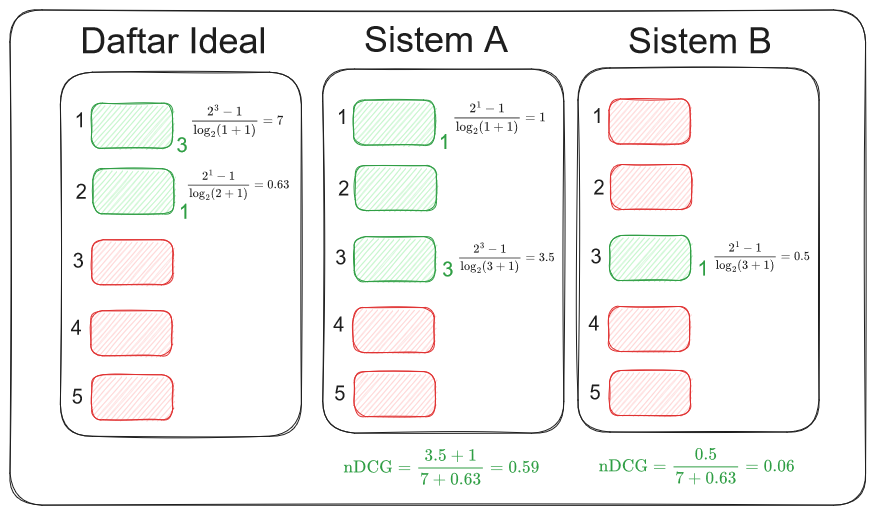
\includegraphics[width=1\textwidth]{assets/pics/contohnDCG.png}
            \caption{\license.}
            \label{fig:ndcg}
        \end{figure}
        \f{Normalized Discounted Cumulative Gain} (nDCG) adalah metrik yang umumnya digunakan untuk mengukur kualitas dari pencarian situs web. Tidak seperti metrik yang telah disebutkan sebelumnya, nDCG dirancang untuk suatu \f{judgements} $r$ yang tak biner. Fungsi $\text{rel}(q, d)$ pada \equ~\ref{eq:rel} berubah menjadi $\text{rel(q,d)}  = r $ ketika menghitung metrik nDCG. \equ~\ref{eq:ndcg-start} hingga \equ~\ref{eq:ndcg-end} menunjukkan cara menghitung nDCG dari suatu kueri $q$ dan barisan $k$ dokumen yang diambil oleh sistem.
        \begin{align}
            \label{eq:ndcg-start}
            \text{nDCG}(q, D_k)\text{@k} &= \frac{\text{DCG}(q, D_k)\text{@k}}{\text{DCG}(q, D_k^{\text{ideal}})\text{@k}} \in [0, 1] \\
            \label{eq:dcg}
            \text{DCG}(q, D_k)\text{@k} &= \sum_{d \in D_k} \frac{2^{\text{rel}(q, d)} - 1}{\log_2(\text{rank}(d, D_k) + 1)} \\
            \label{eq:ndcg-end}
            \text{rank}(d,D_k) &= \text{Posisi } d \text{ dalam } D_k \\
            \text{rel}(q, d) &= r
        \end{align}

        Perhitungan \f{discounted cumulative gain} (DCG) pada \equ~\ref{eq:dcg} dapat dijelaskan menjadi dua faktor, yaitu:
        \begin{enumerate}
            \item faktor $2^{\text{rel}(q, d)} - 1$ menunjukkan bahwa dokumen yang lebih relevan akan memiliki nilai yang lebih tinggi dari dokumen yang kurang relevan untuk posisi dokumen yang sama.
            \item faktor $\frac{1}{\log_2(\text{rank}(d, D_k) + 1)}$ menunjukkan bahwa dokumen yang relevan yang muncul pada peringkat yang lebih tinggi akan memiliki nilai yang lebih tinggi dari dokumen dengan relevansi yang sama, tetapi muncul pada peringkat yang lebih rendah.
        \end{enumerate}
        nilai dari nDCG pada \equ~\ref{eq:ndcg-start} adalah nilai DCG pada barisan dokumen $D_k$ yang dinormalisasi oleh nilai DCG pada barisan dokumen ideal $D_k^{\text{ideal}}$. Barisan dokumen ideal $D_k^{\text{ideal}}$ adalah barisan dokumen yang diurutkan berdasarkan relevansinya dengan kueri $q$.

        Selain itu, jika pada \f{dataset} memiliki \f{judgements} biner, faktor $2^{\text{rel}(q, d)} - 1$ pada \equ~\ref{eq:dcg} dapat diubah menjadi $\text{rel}(q, d)$. Akibatnya, \equ~\ref{eq:dcg} akan menjadi \equ~\ref{eq:dcg-binary}.
        \begin{align}
        \label{eq:dcg-binary}
        \text{DCG}(q, D_k)\text{@k} &= \sum_{d \in D_k} \frac{\text{rel}(q, d)}{\log_2(\text{rank}(d, D_k) + 1)}.
        \end{align}


\section{Pemeringkatan Teks dengan Statistik}
        Untuk mengambil $k$ dokumen dari kumpulan $\mathcal{D}$ diperlukan suatu fungsi skor $s(q, d, \mathcal{D})$ yang mengukur relevansi antara kueri $q$ dan dokumen $d$. dengan mencari skor antara $q$ terhadap semua dokumen pada $\mathcal{D}$, Barisan dokumen $D_k = (d_{i_1}, d_{i_2},\dots, d_{i_k})$ dapat dipilih sehingga $\text{score}(q, d_{i_1}) \geq \text{score}(q, d_{i_2}) \geq \dots \geq \text{score}(q, d_{i_k})$ adalah $k$ dokumen dengan skor tertinggi.
        
        Bagian ini menjelaskan dua fungsi skor stastistik sederhana yang menjadi \f{baseline} ketika membandingkan performa dari model pemeringkatan teks yang lebih kompleks. \sect~\ref{sec:tfidf} menjelaskan fungsi skor statistik yang berdasarkan pada frekuensi kemunculan kata pada dokumen dan kueri. Selanjutnya, \sect~\ref{sec:bm25} membahas fungsi skor statistik yang menjadi standar \f{de facto} dalam pemeringkatan teks.

    \subsection{\f{Term Frequency - Inverse Document Frequency} (TF-IDF)}
    \label{sec:tfidf}
 
    fungsi skor TF-IDF adalah fungsi skor statistik yang menghitung $\text{score}$ antara kueri $q$ dan dokumen $d$ dengan menghitung frekuensi kemunculan kata pada dokumen dan kueri. Untuk suatu kueri $q$, misalkan $T_q= \{t_1, t_2, \dots, t_{L_1}\}$ adalah himpunan kata yang terdapat pada kueri $q$. Selain itu, misalkan juga $T_d = \{t_1, t_2, \dots, t_n\}$ adalah himpunan kata yang terdapat pada dokumen $d$. nilai skor antara $q$ dan $d$ diberikan oleh persamaan \equ~\ref{eq:tfidf-start} sampai \equ~\ref{eq:tfidf-end}.
    \begin{align}
        \label{eq:tfidf-start}
        \mathcal{D} &= \{d_1, d_2, \dots, d_n\} \\
        T_q &= \{t_1, t_2, \dots, t_{L_1}\} \\
        T_d &= \{t_1, t_2, \dots, t_{L_2}\} \\
        \text{tf}(t, d) &= \frac{\text{Count}(t, d)}{|d|} \\
        \text{Count}(t, d) &= \text{jumlah kemunculan } t \text{ dalam } d \\
        \text{df}(t, \mathcal{D}) &= \text{jumlah dokumen pada } \mathcal{D} \text{ yang mengandung } t \\
        \text{idf}(t, \mathcal{D}) &= \begin{cases}
            \log_2\left(\frac{|\mathcal{D}|}{\text{df}(t, \mathcal{D})}\right) & \text{jika } \text{df}(t, \mathcal{D}) > 0 \\
            0 & \text{jika } \text{df}(t, \mathcal{D}) = 0
        \end{cases} \\
        \label{eq:tf-idf-weight}
        \text{TF-IDF}(t, d, \mathcal{D}) &= \text{tf}(t, d) \times \text{idf}(t, \mathcal{D}) \\
        \label{eq:tfidf-end}
        \text{RelevantScore}(q,d,\mathcal{D}) &= \sum_{t \in T_q \cap T_d} \text{tf-idf}(t, d, \mathcal{D})
    \end{align}

    \begin{figure}
        \centering
        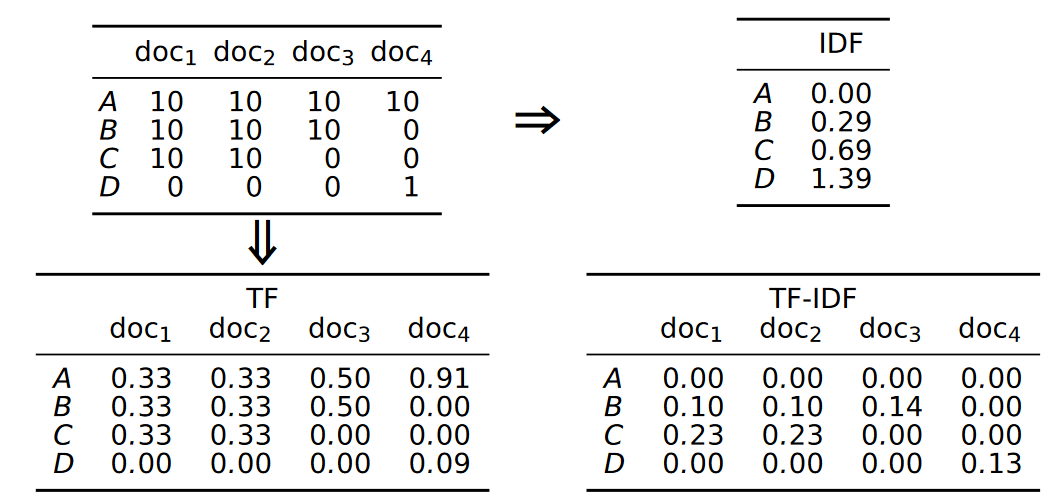
\includegraphics[width=1\textwidth]{assets/pics/tf-idf-matriks.png}
        \caption{\license.}
        \label{fig:tf-idf-matriks}
    \end{figure}

    skor untuk pasangan $(q,d)$ dihitung dengan menjumlahkan skor TF-IDF dari setiap kata yang terdapat pada kueri $q$ dan dokumen $d$. skor TF-IDF dari suatu kata $t$ adalah perkalian antara \f{term frequency} ($\text{tf}(q,d)$) dan \f{inverse document frequency} ($\text{idf}(t,\mathcal{D})$). fungsi skor pada \equ~\ref{eq:tfidf-end} dapat dijelaskan menjadi dua bagian faktor utama berikut:
    \begin{enumerate}
        \item faktor $\text{tf}(t, d)$ menunjukkan bahwa nilai TF-IDF meningkat seiring dengan bertambahnya frekuensi kemunculan kata $t$ pada dokumen $d$.
        \item Faktor $\text{idf}(t, \mathcal{D})$ menunjukkan bahwa nilai TF-IDF meningkat seiring dengan \textit{rarity} dari kata $t$ pada himpunan dokumen $\mathcal{D}$. Akibatnya, kata yang jarang muncul pada himpunan dokumen $\mathcal{D}$ dan muncul pada suatu dokumen tertentu akan menghasilkan skor yang tinggi. Sementara itu, kata-kata yang sering muncul pada koleksi dokumen $\mathcal{D}$ memiliki nilai \textit{downgraded}.
    \end{enumerate}
    \begin{figure}
        \centering
        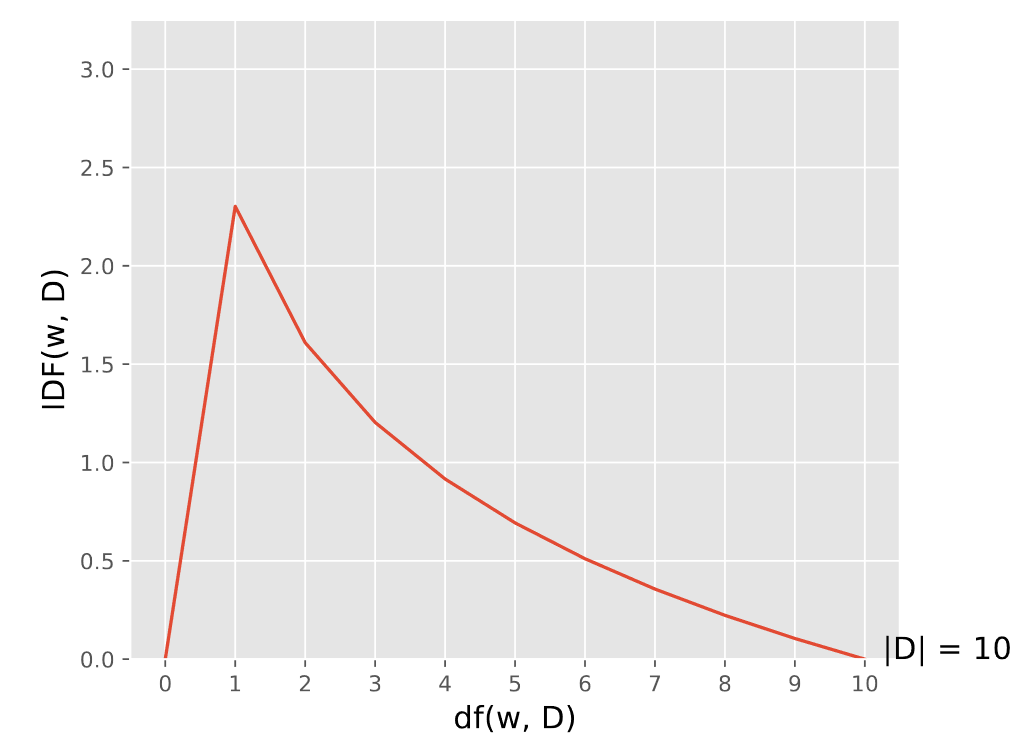
\includegraphics[width=1\textwidth]{assets/pics/idf-graph.png}
        \caption{\license.}
        \label{fig:idf-graph}
    \end{figure}
    
    Kata-kata seperti preposisi atau kata ganti akan menghasilkan skor TF-IDF yang sangat rendah. Hal ini menyiratkan bahwa kata-kata tersebut memiliki sedikit relevansi dalam dokumen dan bisa diabaikan. Di sisi lain, kata-kata yang muncul secara berlebihan dalam satu dokumen tetapi jarang muncul dalam dokumen lainnya akan menghasilkan nilai $\text{tf}(t, d)$ dan $\log \left(\frac{\mathcal{D}}{\text{df}(t, \mathcal{D})}\right)$ yang relatif besar. Dampaknya adalah skor TF-IDF yang dihasilkan juga menjadi signifikan. \pic~\ref{fig:tf-idf-matriks} menunjukkan contoh perhitungan skor TF-IDF untuk suatu kumpulan dokumen dan \pic~\ref{fig:idf-graph} menunjukkan grafik dari fungsi $\text{idf}$.
    
    \subsection{\f{Best Match 25} (BM25)}
    \label{sec:bm25}

    BM25 (\f{Best Match attempt} 25)  merupakan pengembangan dari fungsi skor TF-IDF dengan perbedaan utama pada fungsi nilai yang berkaitan dengan frekuensi kata -- digunakan $\text{score}_{\text{BM25}}(q,d)$ (\equ~\ref{eq:bm25-weight}) daripada $\text{tf}(q,d)$ (\equ~\ref{eq:tf-idf-weight}). Pada fungsi $\text{score}_{\text{BM25}(q,d)}$ terdapat 2 parameter yang dapat diatur, yaitu $b$, dan $k_1$. Setiap parameter mempunyai efek yang berbeda terhadap nilai $\text{score}_{\text{BM25}(q,d)}$ yang dihasilkan. Sebelum menjelaskan efek dari setiap parameter, \equ~\ref{eq:smoothed-idf} hingga \equ~\ref{eq:bm25-end} menunjukkan cara menghitung skor relevansi dari suatu kueri $q$ dan dokumen $d$. 
    \begin{align}
        \label{eq:smoothed-idf}
        \text{idf}_{\text{BM25}}(t, \mathcal{D}) &= \log\left(1+\frac{|\mathcal{D}| - \text{df}(t, \mathcal{D}) + 0.5}{\text{df}(t, \mathcal{D}) + 0.5}\right) \\
        \label{eq:bm25scoring}
        \text{score}_{\text{BM25}}(t,d) &= \frac{\text{tf}(t, d) \times (k_1 + 1)}{\text{tf}(t, d) + k_1 \times (1 - b + b \times \frac{|d|}{\text{avgdl}})} \\
        \label{eq:bm25-weight}
        \text{BM25}(t, d, \mathcal{D}) &= \text{idf}_{\text{BM25}}(t, \mathcal{D}) \times \text{score}_{\text{BM25}}(q,d,\mathcal{D}) \\
        \text{avgdl} &= \text{rata-rata panjang dokumen pada koleksi } \mathcal{D} \\
        \label{eq:bm25-end}
        \text{RelevantScore}(q,d,\mathcal{D}) &= \sum_{t \in T_q \cap T_d} \text{BM25}(t, d, \mathcal{D})
    \end{align}
    \begin{figure}
        \centering
        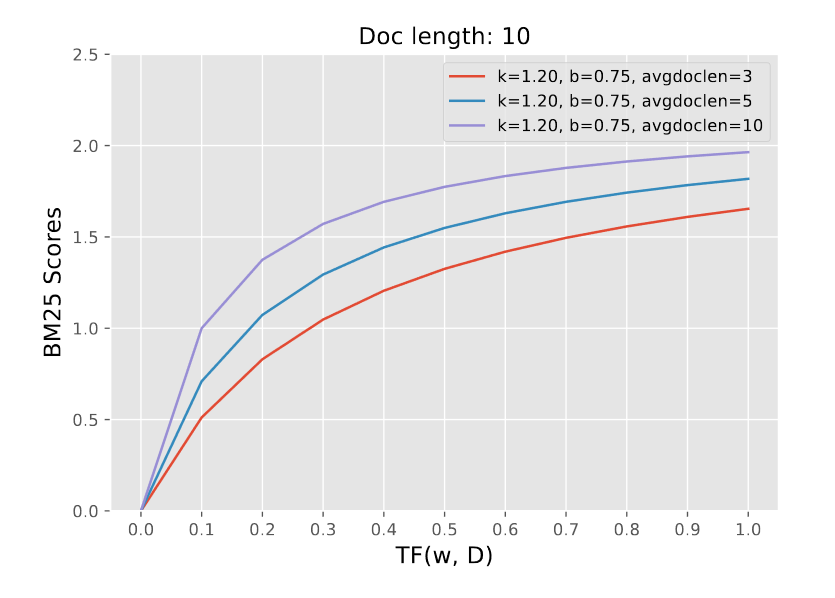
\includegraphics[width=1\textwidth]{assets/pics/effect-bm25-long-doc.png}
        \caption{\license.};
        \label{fig:effect-bm25-long-doc}
    \end{figure}

    \begin{figure}
        \centering
        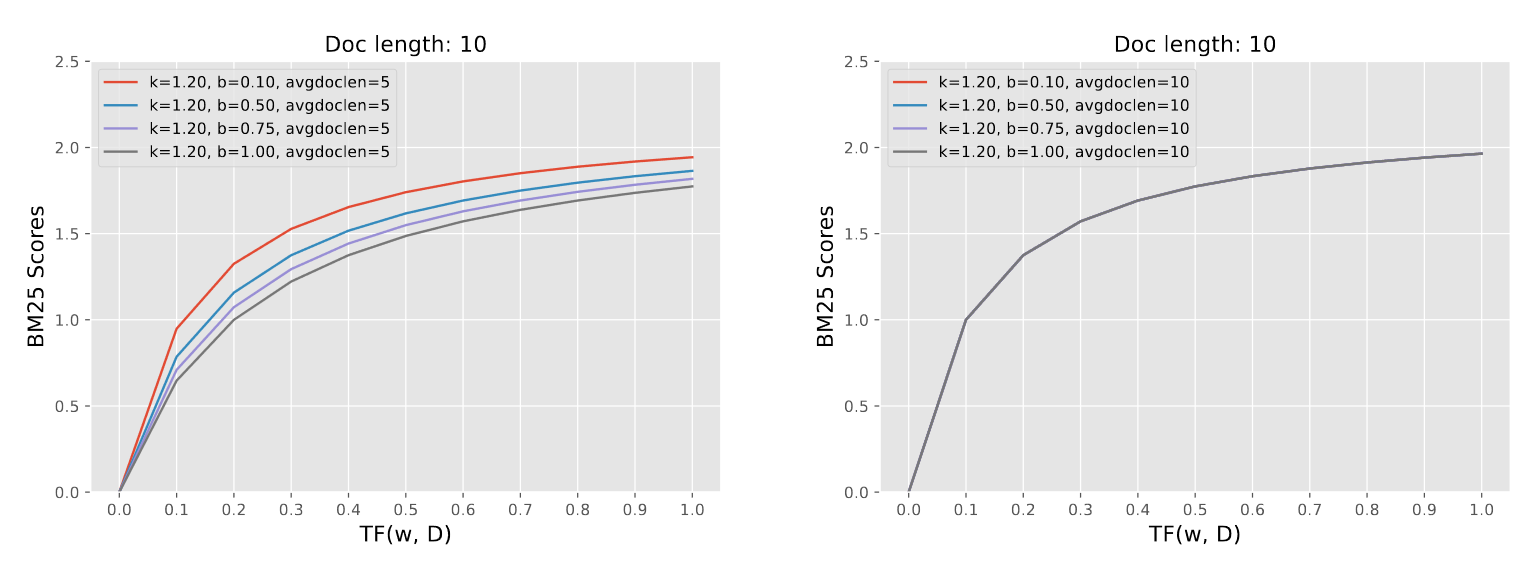
\includegraphics[width=1\textwidth]{assets/pics/effect-bm25-param-b.png}
        \caption{\license.};
        \label{fig:effect-bm25-param-b}
    \end{figure}
    \begin{figure}
        \centering
        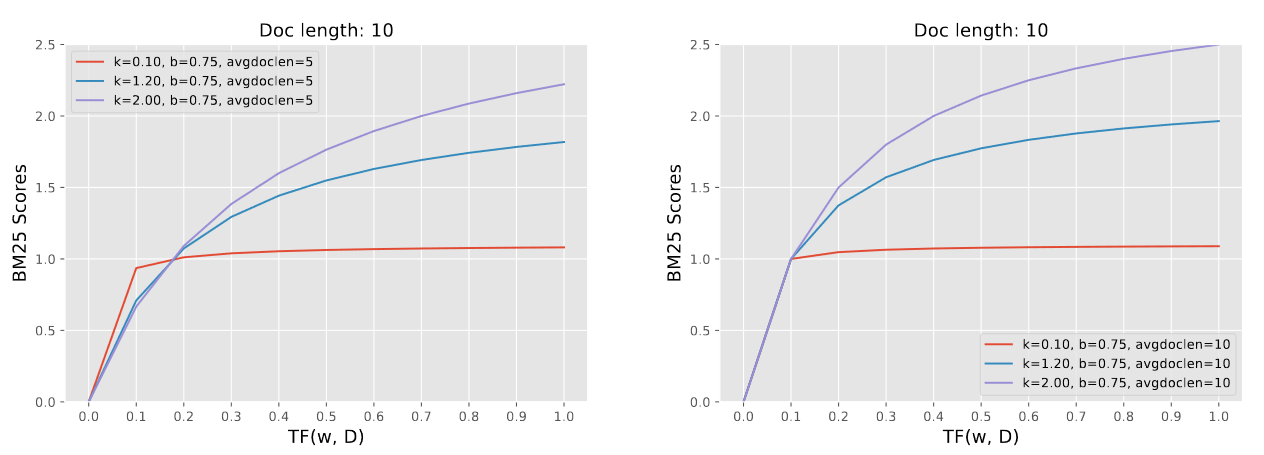
\includegraphics[width=1\textwidth]{assets/pics/effect-bm25-param-k.png}
        \caption{\license.};
        \label{fig:effect-bm25-param-k}
    \end{figure}

    Efek dari masing-masing parameter dan faktor pada $\text{score}_{\text{BM25}}(t,d)$ dapat dijelaskan sebagai berikut:
    \begin{enumerate}
        \item faktor $\frac{|\text{d}|}{\text{avgdl}}$ pada $\frac{\text{tf}(t, d) \times (k_1 + 1)}{\text{tf}(t, d) + k_1 \times \left(1 - b + b \times \textcolor{black}{\frac{|d|}{\text{avgdl}}}\right)}$ men-\f{penalize} skor pada dokumen yang panjangnya lebih besar dari rata-rata panjang dokumen pada himpunan dokumen $\mathcal{D}$. \pic~\ref{fig:effect-bm25-long-doc} Menjukkan efek dari perbedaan nilai $\text{avgdl}$ terhadap skor yang dihasilkan, makin besar rasio $\frac{|d|}{\text{avgdl}}$ makin kecil skor yang dihasilkan.
        \item nilai $b$ menentukan seberapa besar efek dari faktor $\frac{|d|}{\text{avgdl}}$ terhadap skor yang dihasilkan. \pic~\ref{fig:effect-bm25-param-b} Menunjukkjan efek dari perbedaan nilai $b$ terhadap skor yang dihasilkan. Untuk $\frac{|d|}{\text{avgdl}}=1$, Faktor $b$ tidak memiliki pengaruh terhadap skor. Nilai $b$ yang umum dipilih berada pada rentang $[0.5, 0.8]$.
        \item  nilai $k_1$ men-\f{penalize} kemunculan kata $t$ pada dokumen $d$ yang berlebih. \pic~\ref{fig:effect-bm25-param-k} Menunjukkan efek dari perbedaan nilai $k_1$ terhadap skor yang dihasilkan. untuk nilai $k_1$ yang ekstrim, nilai $\text{score}_{\text{BM25}}(t,d)$ hanya menjadi indikator saja dari kemunculan kata $t$ pada dokumen $d$. Nilai $k_1$ yang umum dipilih berada pada rentang $[1.2, 2.0]$.
    \end{enumerate}

    \begin{figure}
        \centering
        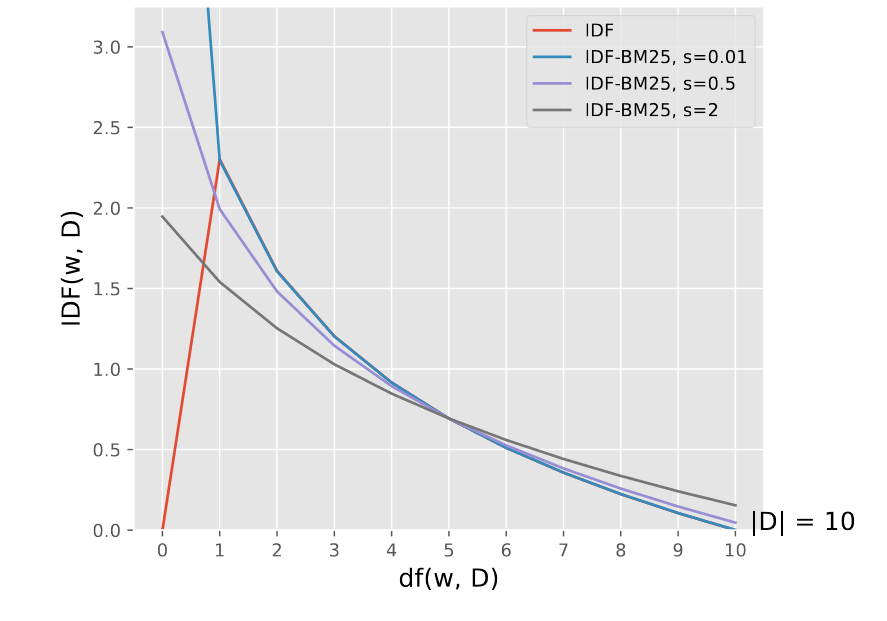
\includegraphics[width=1\textwidth]{assets/pics/smoothed-idf.png}
        \caption{\license.};
        \label{fig:smoothed-idf}
    \end{figure}

    
    Perbedaan \f{minor} lainnya ada pada fungsi $\text{idf}$. Fungsi $\text{idf}$ pada BM25 merupakan versi \f{smoothing} dari $\text{idf}$ dengan tujuan untuk menghindari nilai $\text{idf}$ yang bernilai 0 ketika kata $t$ tidak muncul pada himpunan dokumen $\mathcal{D}$ -- semata-mata untuk konsistensi dengan asumsi bahwa kata $t$ yang tidak muncul pada himpunan dokumen $\mathcal{D}$ memiliki nilai $\text{idf}$ yang paling tinggi. \pic~\ref{fig:smoothed-idf} Menunjukkan Perbedaan antara $\text{idf}_{BM25}$ dan $\text{idf}$. Perbedaan utamanya terjadi ketika $\text{df}(t,\mathcal{D}) = 0$, nilai dari  $\text{idf}_{BM25}$ tak nol dan mengikuti pola yang diharapkan. Ketika $\text{df}(t,\mathcal{D})>0$, nilai dari $\text{idf}_{\text{BM25}}$ dan $\text{idf}$ hampir serupa.

\section{\f{Deep Learning}}

    \begin{figure}
        \centering
        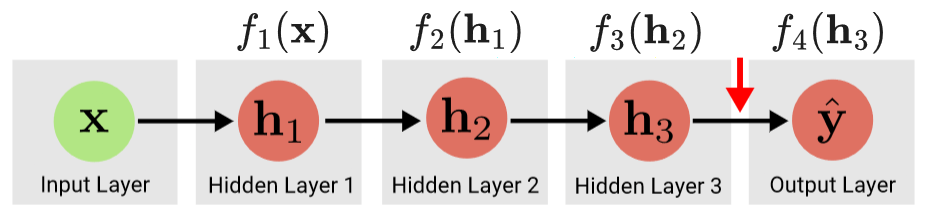
\includegraphics[width=0.50\textwidth]{assets/pics/dag-dl.png}
        \caption{\license.}
        \label{fig:deep-learning-FFN-dag}
    \end{figure}
    Arsitektur \f{Deep learning} merujuk pada model \f{machine learning} yang tersusun dari fungsi-fungsi terturunkan ( yang biasa disebut sebagai \f{layer}), dimana komposisi antara fungsi-fungsi tersebut dapat digambarkan sebagai \f{directed acyclic graph} (DAG) yang memetakan suatu \f{input} ke suatu \f{output}. Biasanya, setiap fungsi dalam Arsitektur \f{Deep learning} memiliki parameter yang ingin diestimasi atau dicari dengan data.
    
    \pic~\ref{fig:deep-learning-FFN-dag} menunjukkan arsitektur deep learning yang sederhana, yaitu \f{feed-forward neural network} (FFN). Pada \pic~\ref{fig:deep-learning-FFN-dag}, \f{input} $\mathbf{x}$ akan dipetakan ke \f{output} $\hat y$ melalui serangkaian fungsi $f_1, f_2, f_3$ yang disebut sebagai \f{layer}. Setiap \f{layer} $f_i$ memiliki parameter $\theta_i$ yang akan diestimasi dengan data. Selain itu, \f{Output} dari \f{layer} $f_i$ akan menjadi \f{input} dari \f{layer} $f_{i+1}$. \f{Output} dari \f{layer} $f_3$ adalah \f{output} dari model. Model pada \pic~\ref{fig:deep-learning-FFN-dag} dapat ditulis sebagai \equ~\ref{eq:deep-learning-FFN-dag}.
    \begin{align}
        \label{eq:deep-learning-FFN-dag}
        \hat y = f_{\text{model}}(\mathbf{x}; \bm{\theta}) &= f_3(f_2(f_1(\mathbf{x}; \bm{\theta}_1); \bm{\theta}_2); \bm{\theta}_3) \\
        \label{eq:deep-learning-FFN-dag-end}
        \text{dengan } \bm{\theta} &= \{\bm{\theta}_1, \bm{\theta}_2, \bm{\theta}_3\}
    \end{align}

    \subsection{\f{Multilayer Perceptron} (MLP)}

    \f{Multi-layer perceptron} (MLP) adalah \f{feed-forward neural network} dengan setiap fungsi $f_i$ adalah fungsi linear yang diikuti oleh fungsi aktivasi non-linear $\phi$  yang diterapkan \f{element-wise} pada setiap \f{output}-nya. \f{hyperparameter} lainnya selain fungsi aktivasi adalah kedalamaan model $L$, dan dimensi \f{output} dari setiap \f{layer} $d_1, d_2, \dots, d_L$.

    Untuk permasalahan regresi dengan \f{input} $\mathbf{x}\in \mathbb{R}^{d_0}$ dan \f{output} $\mathbf{y} \in \mathbb{R}^{d_L}$, \equ~\ref{eq:FFN-regesi-start} hingga \equ~\ref{eq:FFN-regesi-end} menunjukkan arsitektur MLP untuk permasalahan regresi dengan $L$ \f{layer} dan fungsi aktivasi $\phi$.
    \begin{align}
        \label{eq:FFN-regesi-start}
        f_l(\mathbf{x};\mathbf{W}_l, b_l) &= \phi( \mathbf{x} \mathbf{W}_l + \mathbf{b}_l) \in \mathbb{R}^{d_l}, \quad l = 1, 2, \dots, L-1 \\
        f_L(\mathbf{x}) &= \mathbf{x} \mathbf{W}_L + \mathbf{b}_L \in \mathbb{R}^{d_L} \\
        f_{\text{model}}(\mathbf{x};\bm{\theta}) &= f_L(f_{L-1}(\dots f_1(\mathbf{x})) \dots) \\
        \phi(\mathbf{x}) &= \text{fungsi aktivitasi non-linear} \\
        \bm{\theta} &= \{\mathbf{W}_1, \mathbf{b}_1, \mathbf{W}_2, \mathbf{b}_2, \dots, \mathbf{W}_L, \mathbf{b}_L\} \\
        \mathbf{W}_l &= \text{matriks bobot}  \in \mathbb{R}^{d_{l-1} \times d_l} \\
        \label{eq:FFN-regesi-end}
        \mathbf{b}_l &= \text{vektor bias} \in \mathbb{R}^{d_l}
    \end{align} 

    Untuk Permasalahan Klasifikasi Biner dengan \f{input} $\mathbf{x}\in \mathbb{R}^{d_0}$ dan \f{output} $\mathbf{y} \in \{0, 1\}$, \equ~\ref{eq:FFN-klasifikasi-biner-start} hingga \equ~\ref{eq:FFN-klasifikasi-biner-end} menunjukkan arsitektur MLP untuk permasalahan klasifikasi biner.
    \begin{align}
        \label{eq:FFN-klasifikasi-biner-start}
        f_{\text{model}}(\mathbf{x};\bm{\theta}) &= f_L(f_{L-1}(\dots f_1(\mathbf{x})) \dots), \\
        f_L(\mathbf{x}) &= \sigma(\mathbf{x} \mathbf{W}_L + \mathbf{b}_L \in \mathbb{R}), \\
        \sigma(x) &= \frac{1}{1 + e^{x}} \in (0, 1), \\
        \text{decision}(\mathbf{x};\bm{\theta}) &= \begin{cases}
        1 & \text{jika } f(\mathbf{x};\bm{\theta}) \geq \text{threshold} \\
        0 & \text{jika } f(\mathbf{x};\bm{\theta}) < \text{threshold} \\
        \end{cases}, \\
        \label{eq:FFN-klasifikasi-biner-end}
        \text{threshold}&\in [0, 1].
    \end{align}

    Perbedaan utama antara MLP untuk permasalahan regresi dan klasifikasi adalah fungsi aktivasi pada \f{output layer}. Pada permasalahan regresi, fungsi aktivasi pada \f{output layer} adalah fungsi identitas, sedangkan pada permasalahan klasifikasi, fungsi aktivasi pada \f{output layer} adalah fungsi \f{sigmoid}. Tujuan pengunaan fungsi \f{sigmoid} pada permasalahan klasifikasi adalah untuk memastikan bahwa \f{output} dari model berada pada rentang $[0, 1]$, nilai tersebut dapat diinterpretasikan sebagai probabilitas $\mathbf{x}$ termasuk pada kelas positif. Selain itu, \f{threshold} pada \equ~\ref{eq:FFN-klasifikasi-biner-end} digunakan untuk menentukan kelas dari $\mathbf{x}$.

    \subsection{Fungsi Aktivasi}

    Fungsi Aktivasi pada setiap fungsi $f_i$ pada \f{multilayer perceptron} digunakan untuk menambahkan non-linearitas pada model. Sebab, tanpa adanya fungsi aktivasi non-linear, model \f{multilayer perceptron} akan menjadi model linear. Selain itu, fungsi aktivasi juga biasanya adalah fungsi yang terturunkan, meskipun tidak perlu terturunkan disetiap titik. \tab~\ref{tab:activation-function} menunjukkan beberapa fungsi aktivasi yang sering digunakan pada \f{multilayer perceptron}. \pic~\ref{fig:activation-function} menunjukkan grafik dari fungsi aktivasi pada \tab~\ref{tab:activation-function} dan turunannya.
    \begin{table}
        \centering
        \caption{Beberapa fungsi aktivasi yang sering digunakan pada \f{multilayer perceptron}.}
        \label{tab:activation-function}
        \begin{tabular}{|c|c|}
            \hline
            \textbf{Fungsi Aktivasi} & \textbf{Persamaan} \\
            \hline
            \hline
            Sigmoid & $\sigma(x) = \frac{1}{1 + e^{-x}}$ \\
            \hline
            Tanh & $\tanh(x) = \frac{e^x - e^{-x}}{e^x + e^{-x}}$ \\
            \hline
            ReLU & $\text{ReLU}(x) = \max(0, x)$ \\
            \hline
            Leaky ReLU & $\text{LeakyReLU}(x) = \max(\alpha x, x), \alpha \in [0, 1]$ \\
            \hline
        \end{tabular}
    \end{table}
    \begin{figure}
        \centering
        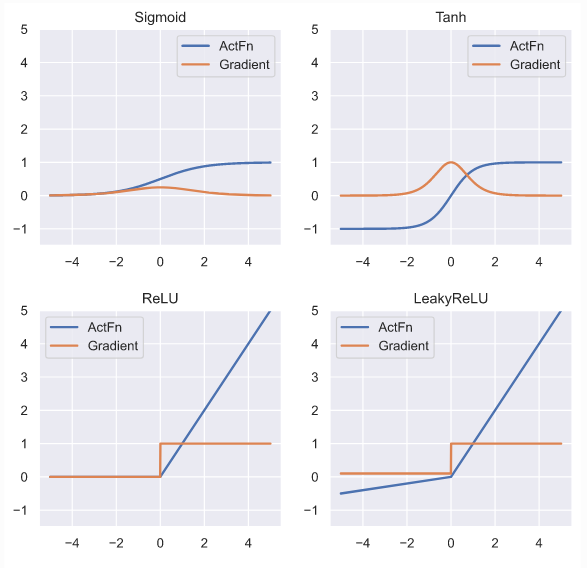
\includegraphics[width=1\textwidth]{assets/pics/act_function.png}
        \caption{\license.}
        \label{fig:activation-function}
    \end{figure}


    \subsection{Fungsi \f{Loss}}
    Misalkan $\mathcal{D} = \{(\mathbf{x}_1, \mathbf{y}_1), (\mathbf{x}_2, \mathbf{y}_2), \dots, (\mathbf{x}_n, \mathbf{y}_n)\}$ adalah \f{dataset} yang terdiri dari $n$ pasangan \f{input} dan \f{output}. Parameter $\bm{\theta}$ pada $f_{\text{model}}$ diestimasi dengan melakukan \f{fitting} pada \f{dataset} $\mathcal{D}$. Untuk melakukan \f{fitting} pada \f{dataset} $\mathcal{D}$, diperlukan suatu fungsi \f{loss} yang mengukur seberapa baik hasil pemetaan $f_{\text{model}}$ pada \f{input} $\mathbf{x}_i$ terhadap \f{output} $\mathbf{y}_i$. Meskipun sembarang fungsi yang terturunkan dapat digunakan sebagai fungsi \f{loss}, namun pemilihan fungsi \f{loss} berdasarkan \f{maximum likelihood estimation} (MLE) lebih disarankan. 
    
    Untuk permasalahan klasifikasi biner, fungsi \f{loss} yang sering digunakan adalah \f{binary cross entropy} (BCE) seperti yang ditinjukkan pada \equ~\ref{eq:bce}. Penurunan fungsi \f{loss} BCE dengan mengikuti prinsip MLE yang akan dijelaskan pada bagian berikut.
    
    Misalkan $y_i \mid \mathbf{x}$ mengikuti distribusi bernouli dengan parameter $\text{p} = f_{\text{model}}(\mathbf{x};\bm{\theta})$ yang saling independen antara satu sama lainnya. \equ~\ref{eq:definisi-random-variable} menunjukkan definisi dari $y_i \mid \mathbf{x}$.
    \begin{align}
        \label{eq:definisi-random-variable}
        y_i \mid \mathbf{x} &\overset{\text{iid}}{\sim} \text{Bernoulli}(f_{\text{model}}(\mathbf{x};\bm{\theta})) \\
        p(y_i \mid \mathbf{x}) &= f_{\text{model}}(\mathbf{x};\bm{\theta})^{y_i} (1 - f_{\text{model}}(\mathbf{x};\bm{\theta}))^{1 - y_i} 
    \end{align} 

    Fungsi $\f{likelihood}$ dari $\bm{\theta}$ terhadap \f{dataset} $\mathcal{D}$ dapat ditulis sebagai berikut:
    \begin{align}
        \mathcal{L}(\bm{\theta}) &= \prod_{i=1}^N p(y_i \mid \mathbf{x}_i; \bm{\theta}).
    \end{align}

    Dengan prinsip MLE, parameter $\bm{\theta}$ yang dicari adalah parameter $\bm{\theta}$ yang memaksimalkan fungsi \f{likelihood} $\mathcal{L}(\bm{\theta})$,
    \begin{align}
        \bm{\theta}_{\text{MLE}} &= \arg\max_{\bm{\theta}} \mathcal{L}(\bm{\theta}).
    \end{align}

    Untuk mempermudah perhitungan, fungsi \f{likelihood} diubah menjadi negatif \f{log-likelihood} $\mathcal{\ell}(\bm{\theta})$, sehingga permasalahan optimasi dapat ditulis seperti \equ~\ref{eq:log-likelihood} hingga \equ~\ref{eq:log-likelihood-end}.
    \begin{align}
        \label{eq:log-likelihood}
        \ell{(\bm{\theta})} &= -\log\mathcal{L}(\bm{\theta}), \\
        &= -\sum_{i=1}^N \log\left(p(y_i \mid \mathbf{x}_i; \bm{\theta})\right), \\
        \label{eq:log-likelihood-end}
        \bm{\theta}_{\text{MLE}} &= \arg\min_{\bm{\theta}} \ell(\bm{\theta}).
    \end{align} 

    Dengan mengganti $p(y_i \mid \mathbf{x}_i; \bm{\theta})$ dengan fungsi distribusi-nya, maka fungsi \f{loss} yang digunakan untuk permasalahan klasifikasi biner adalah \f{binary cross entropy} (BCE) seperti pada \equ~\ref{eq:bce}. \pic~\ref{fig:dl-training-graph-dag} mengilustrasikan \f{directed acyclic graph} (DAG) dari model ketika proses pelatihan dilakukan.
    \begin{align}
        \bm{\theta}_{\text{MLE}} &= \arg\min_{\bm{\theta}}\sum_{i=1}^{N}\underbrace{-y_i \log\left(f_{\text{model}}(\mathbf{x}_i; \bm{\theta})\right) - (1 - y_i) \log\left(1 - f_{\text{model}}(\mathbf{x}_i; \bm{\theta})\right)}_{\text{Binary Cross Entropy Loss } L(y_i, f_{\text{model}}(\mathbf{x}_i; \bm{\theta}))}, \\
        \label{eq:bce} 
        L(y_i, f_{\text{model}}(\mathbf{x}_i; \bm{\theta})) &= -y_i \log\left(f_{\text{model}}(\mathbf{x}_i; \bm{\theta})\right) - (1 - y_i) \log\left(1 - f_{\text{model}}(\mathbf{x}_i; \bm{\theta})\right).
    \end{align}
    \begin{figure}
        \centering
        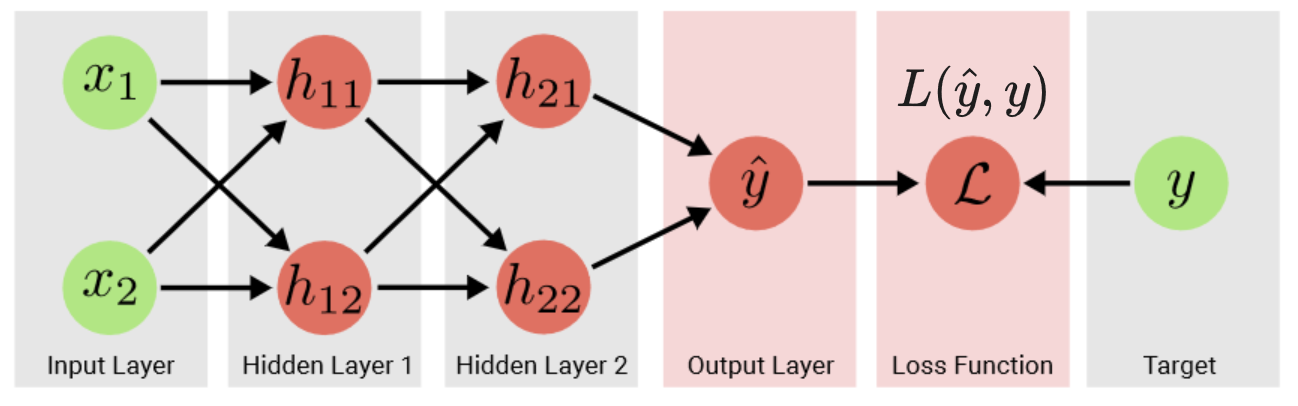
\includegraphics[width=1\textwidth]{assets/pics/dl-training-graph.png}
        \caption{\license.}
        \label{fig:dl-training-graph-dag}
    \end{figure}

    Untuk mendapatkan $f_\text{model}$ dengan performa yang baik, dibutuhkan model dengan nilai $\ell(\bm{\theta})$ seminimum mungkin. Namun, pencarian $\bm{\theta}$ sehingga $ \ell (\bm{\theta})$ minumum secara analitik tidak dapat dilakukan karena non-linearitas yang ada pada model, dengan kata lain solusi dari $\nabla_{\bm{\theta}} \ell(\bm{\theta}) = 0$ tidak dapat dicari secara analitik. Sebagai gantinya, pencarian $\bm{\theta}$ dilakukan secara numerik dengan menggunakan metode \f{gradient descent} yang akan dijelaskan pada bagian selanjutnya.
    
    \subsection{\f{Backpropagation}}

    \subsection{\f{Optimasi} Parameter}

    \f{Gradient Descent} adalah metode numerik yang digunakan untuk mencari nilai $\bm{\theta}$ yang meminimalkan fungsi \f{loss} $\ell(\bm{\theta})$. Pada metode \f{gradient descent}, nilai $\bm{\theta}$ diupdate secara iteratif dengan mengikuti arah negatif dari \f{gradient} $\nabla_{\bm{\theta}} \mathcal{L}(\bm{\theta})$ yang menunjukkan arah dari penurunan fungsi \f{loss} $\mathcal{L}(\bm{\theta})$. \equ~\ref{eq:gradient-descent} menunjukkan algoritma \f{gradient descent}.
    \begin{align}
        \mathcal{D} &= \{(\mathbf{x}_1, y_1), (\mathbf{x}_2, y_2), \dots, (\mathbf{x}_n, y_n)\} \\
        \label{eq:gradient-descent}
        \bm{\theta}^{(t+1)} &= \bm{\theta}^{(t)} - \eta \frac{1}{n} \sum_{i=1}^{n} \nabla_{\bm{\theta}} L(y_i, f_{\text{model}}(\mathbf{x}_i; \bm{\theta}^{(t)})), \\
        \text{dengan } \eta &\in \mathbb{R}^+ \text{ adalah \f{learning rate}}.
    \end{align}

    Perlu diketahui bahwa pada metode \f{gradient descent} memperbarui parameter dengan mengambil rata-rata \f{gradient} dari semua data pada \f{dataset} pelatihan $\mathcal{D}$. Hal ini menciptakan masalah ketika model menggunakan banyak parameter dan jumlah data pada \f{datasets} latih besar, yaitu komputasi \f{forward pass} dan \f{backward pass} menjadi sangat mahal dan diperlukan memori yang besar untuk menyimpan gradient dari semua data pada \f{dataset} latih. Untuk mengatasi masalah tersebut, digunakan metode \f{stochastic gradient descent} (SGD) dimana setiap \f{update} dari parameter $\bm{\theta}$ dihitung dengan mengambil rata-rata \f{gradient} dari sebagian data pada \f{dataset} $\mathcal{B}\subseteq\mathcal{D}$. \equ~\ref{eq:stochastic-gradient-descent} menunjukkan algoritma \f{stochastic gradient descent}.
    \begin{align}
        \mathcal{B} = \{(\mathbf{x}_{i_1}, y_{i_1}), (\mathbf{x}_{i_2}, y_{i_2}), \dots, (\mathbf{x}_{i_b}, y_{i_b})\} &\subseteq \mathcal{D}, \mid \mathcal{B} \mid \ll \mid \mathcal{D} \mid, \\
        \label{eq:stochastic-gradient-descent-approx}
        \nabla_{\bm{\theta}}{\mathcal{L_B}}(\bm{\theta}) &= 
         \frac{1}{b} \sum_{i=1}^{b} \nabla_{\bm{\theta}} L(y_{i}, f_{\text{model}}(\mathbf{x}_{i}; \bm{\theta})), \\
        \label{eq:stochastic-gradient-descent}
        \bm{\theta}^{(t+1)} &= \bm{\theta}^{(t)} - \eta \nabla_{\bm{\theta}} \mathcal{L_B}(\bm{\theta}^{(t)}).
    \end{align}

    \f{hyperparameter} \f{learning rate} mengatur laju dari perubahan parameter $\bm{\theta}$ pada setiap iterasi pembaruan. Dengan demikian, pemilihan \f{learning rate} berpengaruh terhadap kekonvergenan optimasi yang dilakukan. Jika \f{learning rate} yang digunakan terlalu kecil, model membutuhkan waktu yang jauh lebih lama untuk mencapai nilai parameter $\bm{\theta}$ yang optimal. Di lain sisi, pemilihan \f{learning rate} yang terlalu besar dapat membuat model tidak dapat menemukan nilai parameter $\bm{\theta}$ yang optimal. \pic~\ref{fig:learning-rate-bad} mengilustrasikan proses pembaruan parameter $\bm{\theta}$ dengan \f{learning rate} yang terlalu kecil dan terlalu besar, dan \pic~\ref{fig:learning-rate-good} mengilustrasikan proses pembaruan parameter $\bm{\theta}$ dengan \f{learning rate} yang baik.
\begin{figure}
    \centering
    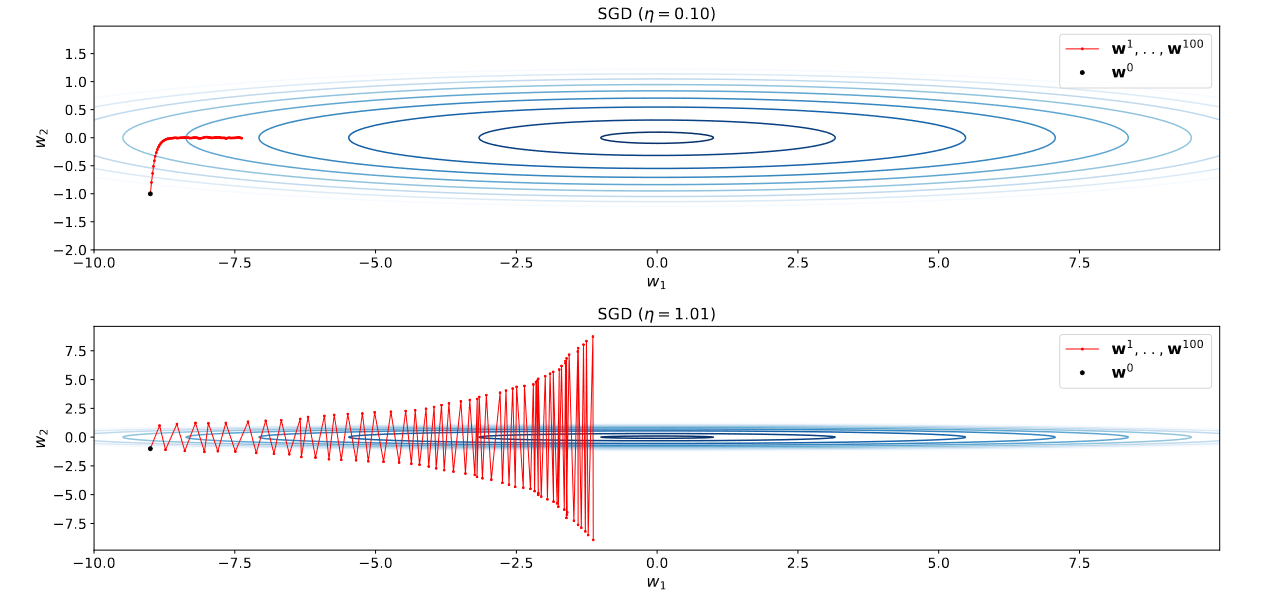
\includegraphics[width=1\textwidth]{assets/pics/learning-rate-bad.png}
    \caption{\license.}
    \label{fig:learning-rate-bad}
\end{figure}
\begin{figure}
    \centering
    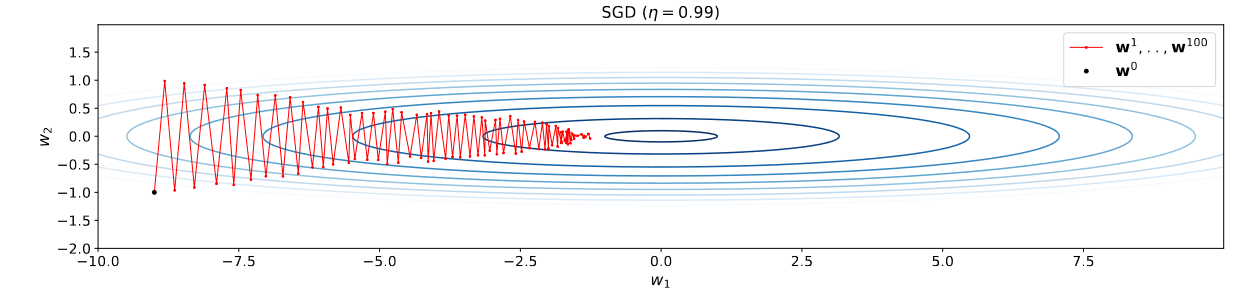
\includegraphics[width=1\textwidth]{assets/pics/learning-rate-good.png}
    \caption{\license.}
    \label{fig:learning-rate-good}
\end{figure}

    Untuk mempercepat proses pembaruan parameter $\bm{\theta}$, digunakan metode \f{stochastic gradient descent} dengan momentum untuk mengurangi osilasi pada proses pembaruan parameter. daripada memperbarui parameter $\bm{\theta}$ dengan gradien pada iterasi sekarang saja, metode \f{stochastic gradient descent} dengan momentum memperbarui parameter $\bm{\theta}$ dengan gradien pada iterasi sekarang dan gradien pada iterasi sebelumnya. gradien yang digunakan untuk melakukan pembaruan parameter $\bm{\theta}$ \f{exponential moving average} dari gradien pada iterasi sekarang dan gradien pada iterasi sebelumnya. \equ~\ref{eq:sgd-momentum} menunjukkan algoritma \f{stochastic gradient descent} dengan momentum dan \pic~\ref{fig:sgd-momentum} mengilustrasikan pembaruan parameter $\bm{\theta}$ dengan momentum.
\begin{figure}
    \centering
    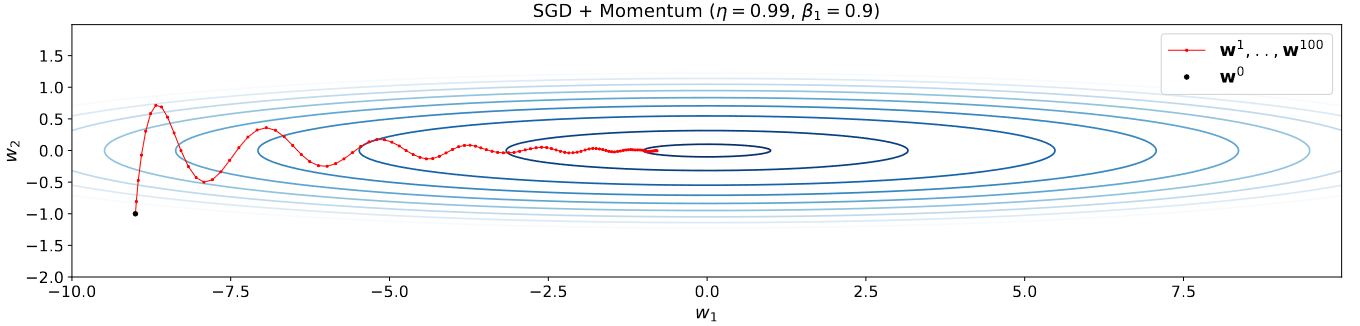
\includegraphics[width=1\textwidth]{assets/pics/sgd-momentum.png}
    \caption{\license.}
    \label{fig:sgd-momentum}
\end{figure}

\begin{align}
    \label{eq:sgd-momentum}
    \bm{\theta}^{(t+1)} &= \bm{\theta}^{(t)} - \eta m^{(t+1)}, \\
    \bm{m}^{(t+1)} &= \beta_1 \bm{m}^{(t)} + (1 - \beta_1) \nabla_{\bm{\theta}} L_{\mathcal{B}}(\bm{\theta}^{(t)}).
\end{align}


    Metode lainnya yang dapat digunakan untuk mempercepat proses pembaruan parameter $\bm{\theta}$ adalah metode \f{adaptive learning rate}. Metode \f{adaptive learning rate} mengubah \f{learning rate} pada setiap parameter $\bm{\theta}$ dengan membagi \f{learning rate} awal dengan \f{moving average} dari kuadrat gradien -- biasanya disebut sebagai \f{running variance} -- pada parameter $\bm{\theta}$ tersebut. Pembagian antara gradien dan \f{running variance} tersebut dilakukan secara \f{element-wise}. \equ~\ref{eq:rmsprop} menunjukkan algoritma \f{stochastic gradient descent} dengan \f{adaptive learning rate} dan \pic~\ref{fig:rmsprop} menngilustrasikan pembaruan parameter $\bm{\theta}$ dengan \f{adaptive learning rate}.
\begin{figure}
    \centering
    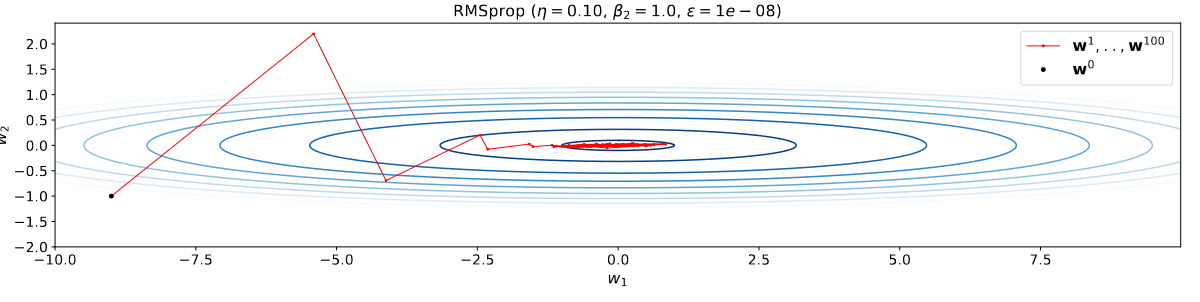
\includegraphics[width=1\textwidth]{assets/pics/RMSPROP.png}
    \caption{\license.}
    \label{fig:rmsprop}
\end{figure}
\begin{align}
    \label{eq:rmsprop}
    \bm{\theta}^{(t+1)} &= \bm{\theta}^{(t)} - \frac{\eta \nabla_{\bm{\theta}} L_{\mathcal{B}}(\bm{\theta}^{(t)}).}{\sqrt{v^{(t+1)}} + \epsilon}, \\
    \bm{v}^{(t+1)} &= \beta_2 \bm{v}^{(t)} + (1 - \beta_2) \nabla_{\bm{\theta}} L_{\mathcal{B}}(\bm{\theta}^{(t)})\odot \nabla_{\bm{\theta}} L_{\mathcal{B}}(\bm{\theta}^{(t)}).
\end{align}

faktor $\epsilon$ yang ditambahkan pada \equ~\ref{eq:rmsprop} digunakan untuk menghindari pembagian dengan nol pada awal iterasi karena inisialiasi awal vektor $\bm{v}^{(0)}$ adalah nol.

Terakhir, metode optimasi \f{Adaptive Moment Estimation} (Adam) menggabungkan metode \f{stochastic gradient descent} dengan momentum dan \f{adaptive learning rate}. \equ~\ref{eq:adam} menunjukkan algoritma \f{stochastic gradient descent} dengan Adam dan \pic~\ref{fig:adam} mengilustrasikan pembaruan parameter $\bm{\theta}$ dengan Adam. \equ~\ref{eq:adam} menunjukkan persamaan dari metode optimasi Adam dan \pic~\ref{fig:adam} mengilustrasikan pembaruan parameter $\bm{\theta}$ dengan Adam.
\begin{figure}
    \centering
    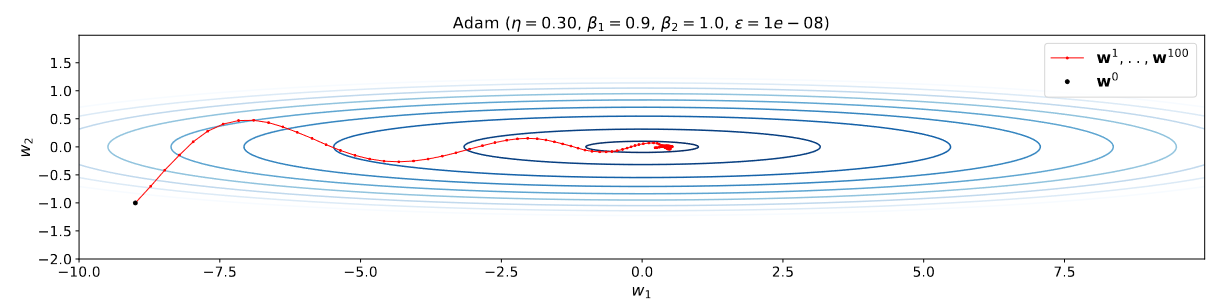
\includegraphics[width=1\textwidth]{assets/pics/adam.png}
    \caption{\license.}
    \label{fig:adam}
\end{figure}
\begin{align}
    \label{eq:adam}
    \bm{\theta}^{(t+1)} &= \bm{\theta}^{(t)} - \frac{\eta \hat{\mathbf{m}}^{(t+1)}}{\sqrt{\hat{\mathbf{v}}^{(t+1)}} + \epsilon}, \\
    \label{eq:adam-momemntum-with-bias-correction}
    \hat{\mathbf{m}}^{(t+1)} &= \frac{\mathbf{m}^{(t+1)}}{1 - \beta_1}, \\
    \label{eq:adam-running-variance-with-bias-correction}
    \hat{\mathbf{v}}^{(t+1)} &= \frac{\mathbf{v}^{(t+1)}}{1 - \beta_2}, \\
    \mathbf{m}^{(t+1)} &= \beta_1 \mathbf{m}^{(t)} + (1 - \beta_1) \nabla_{\bm{\theta}} L_{\mathcal{B}}(\bm{\theta}^{(t)}), \\
    \mathbf{v}^{(t+1)} &= \beta_2 \mathbf{v}^{(t)} + (1 - \beta_2) \left(\nabla_{\bm{\theta}} L_{\mathcal{B}}(\bm{\theta}^{(t)})\odot \nabla_{\bm{\theta}} L_{\mathcal{B}}(\bm{\theta}^{(t)})\right).
\end{align}

Alasan dilakukan pembagian dengan $(1-\beta_1)$ dan $(1-\beta_2)$ \equ~\ref{eq:adam-momemntum-with-bias-correction} dan \equ~\ref{eq:adam-running-variance-with-bias-correction} adalah untuk menghilangkan bias pada \f{momentum} dan \f{running variance} pada awal iterasi.

\subsection{Inisialisasi Bobot}
    \label{sec:kaiminginit}

\section{Pembelajaran Representasi}

    \subsection{Fungsi \f{Loss} pada Pembelajaran Representasi}













        

